  %==============================================================================
% tento soubor pouzijte jako zaklad
% this file should be used as a base for the thesis
% (c) 2008 Michal Bidlo
% E-mail: bidlom AT fit vutbr cz
% Šablonu upravil / template edited by: Ing. Jaroslav Dytrych, dytrych@fit.vutbr.cz
%==============================================================================
% kodovaní: UTF-8 (zmena prikazem iconv, recode nebo cstocs)
% encoding: UTF-8 (you can change it by command iconv, recode or cstocs)
%------------------------------------------------------------------------------
% zpracování / processing: make, make pdf, make clean
%==============================================================================
% Soubory, které je nutné upravit: / Files which have to be edited:
%   xcoufa08-Pohled-na-stav-JUnit-pro-testovanou-instanci-eclipse-20-literatura-bibliography.bib - literatura / bibliography
%   xcoufa08-Pohled-na-stav-JUnit-pro-testovanou-instanci-eclipse-01-kapitoly-chapters.tex - obsah práce / the thesis content
%   xcoufa08-Pohled-na-stav-JUnit-pro-testovanou-instanci-eclipse-30-prilohy-appendices.tex - přílohy / appendices
%==============================================================================
%\documentclass[]{fitthesis} % bez zadání - pro začátek práce, aby nebyl problém s překladem
%\documentclass[english]{fitthesis} % without assignment - for the work start to avoid compilation problem
\documentclass[zadani]{fitthesis} % odevzdani do wisu - odkazy jsou barevné
%\documentclass[english,zadani]{fitthesis} % for submission to the IS FIT - links are color
%\documentclass[zadani,print]{fitthesis} % pro tisk - odkazy jsou černé
%\documentclass[english,zadani,print]{fitthesis} % for the print - links are black
% * Je-li prace psana v anglickem jazyce, je zapotrebi u tridy pouzit 
%   parametr english nasledovne:
%   If thesis is written in english, it is necessary to use 
%   parameter english as follows:
%      \documentclass[english]{fitthesis}
% * Je-li prace psana ve slovenskem jazyce, je zapotrebi u tridy pouzit 
%   parametr slovak nasledovne:
%      \documentclass[slovak]{fitthesis}

% Základní balíčky jsou dole v souboru šablony fitthesis.cls
% Basic packages are at the bottom of template file fitthesis.cls
%zde muzeme vlozit vlastni balicky / you can place own packages here
\usepackage[export]{adjustbox}
%\usepackage{enumitem}
%---rm---------------
\renewcommand{\rmdefault}{lmr}%zavede Latin Modern Roman jako rm / set Latin Modern Roman as rm
%---sf---------------
\renewcommand{\sfdefault}{qhv}%zavede TeX Gyre Heros jako sf
%---tt------------
\renewcommand{\ttdefault}{lmtt}% zavede Latin Modern tt jako tt

% vypne funkci šablony, která automaticky nahrazuje uvozovky,
% aby nebyly prováděny nevhodné náhrady v popisech API apod.
% disables function of the template which replaces quotation marks
% to avoid unnecessary replacements in the API descriptions etc.
\csdoublequotesoff

% =======================================================================
% balíček "hyperref" vytváří klikací odkazy v pdf, pokud tedy použijeme pdflatex
% problém je, že balíček hyperref musí být uveden jako poslední, takže nemůže
% být v šabloně
% "hyperref" package create clickable links in pdf if you are using pdflatex.
% Problem is that this package have to be introduced as the last one so it 
% can not be placed in the template file.
\ifWis
\ifx\pdfoutput\undefined % nejedeme pod pdflatexem / we are not using pdflatex
\else
  \usepackage{color}
  \usepackage[unicode,colorlinks,hyperindex,plainpages=false,pdftex]{hyperref}
  \definecolor{links}{rgb}{0.4,0.5,0}
  \definecolor{anchors}{rgb}{1,0,0}
  \def\AnchorColor{anchors}
  \def\LinkColor{links}
  \def\pdfBorderAttrs{/Border [0 0 0] }  % bez okrajů kolem odkazů / without margins around links
  \pdfcompresslevel=9
\fi
\else % pro tisk budou odkazy, na které se dá klikat, černé / for the print clickable links will be black
\ifx\pdfoutput\undefined % nejedeme pod pdflatexem / we are not using pdflatex
\else
  \usepackage{color}
  \usepackage[unicode,colorlinks,hyperindex,plainpages=false,pdftex,urlcolor=black,linkcolor=black,citecolor=black]{hyperref}
  \definecolor{links}{rgb}{0,0,0}
  \definecolor{anchors}{rgb}{0,0,0}
  \def\AnchorColor{anchors}
  \def\LinkColor{links}
  \def\pdfBorderAttrs{/Border [0 0 0] } % bez okrajů kolem odkazů / without margins around links
  \pdfcompresslevel=9
\fi
\fi
% Řešení problému, kdy klikací odkazy na obrázky vedou za obrázek
% This solves the problems with links which leads after the picture
\usepackage[all]{hypcap}

% Informace o práci/projektu / Information about the thesis
%---------------------------------------------------------------------------
\projectinfo{
  %Prace / Thesis
  project=BP,            %typ prace BP/SP/DP/DR  / thesis type (SP = term project)
  year=2017,             %rok odevzdání / year of submission
  date=\today,           %datum odevzdani / submission date
  %Nazev prace / thesis title
  title.cs={Pohled na stav JUnit pro testovanou instanci Eclipse},  %nazev prace v cestine ci slovenstine (dle zadani) / thesis title in czech language (according to assignment)
  title.en={JUnit Status View for Tested Eclipse Instance}, %nazev prace v anglictine / thesis title in english
  %Autor / Author
  author={Martin Coufal},   %cele jmeno a prijmeni autora / full name and surname of the author
  author.name={Martin},   %jmeno autora (pro citaci) / author name (for reference) 
  author.surname={Coufal},   %prijmeni autora (pro citaci) / author surname (for reference) 
  %author.title.p=Bc., %titul pred jmenem (nepovinne) / title before the name (optional)
  %author.title.a=PhD, %titul za jmenem (nepovinne) / title after the name (optional)
  %Ustav / Department
  department=UIFS, % doplnte prislusnou zkratku dle ustavu na zadani: UPSY/UIFS/UITS/UPGM
  %                  fill in appropriate abbreviation of the department according to assignment: UPSY/UIFS/UITS/UPGM
  %Skolitel / supervisor
  supervisor=Zbyněk Křivka, %cele jmeno a prijmeni skolitele / full name and surname of the supervisor
  supervisor.name={Zbyněk},   %jmeno skolitele (pro citaci) / supervisor name (for reference) 
  supervisor.surname={Křivka},   %prijmeni skolitele (pro citaci) / supervisor surname (for reference) 
  supervisor.title.p=Ing.,   %titul pred jmenem (nepovinne) / title before the name (optional)
  supervisor.title.a={Ph.D.},    %titul za jmenem (nepovinne) / title after the name (optional)
  %Klicova slova, abstrakty, prohlaseni a podekovani je mozne definovat 
  %bud pomoci nasledujicich parametru nebo pomoci vyhrazenych maker (viz dale)
  %Keywords, abstracts, declaration and acknowledgement can be defined by following 
  %parameters or using dedicated macros (see below)
  %===========================================================================
  %Klicova slova / keywords
  %keywords.cs={Klíčová slova v českém jazyce.}, %klicova slova v ceskem ci slovenskem jazyce
  %                                              keywords in czech or slovak language
  %keywords.en={Klíčová slova v anglickém jazyce.}, %klicova slova v anglickem jazyce / keywords in english
  %Abstract
  %abstract.cs={Výtah (abstrakt) práce v českém jazyce.}, % abstrakt v ceskem ci slovenskem jazyce
  %                                                         abstract in czech or slovak language
  %abstract.en={Výtah (abstrakt) práce v anglickém jazyce.}, % abstrakt v anglickem jazyce / abstract in english
  %Prohlaseni / Declaration
  %declaration={Prohlašuji, že jsem tuto bakalářskou práci vypracoval samostatně pod vedením pana ...},
  %Podekovani (nepovinne) / Acknowledgement (optional)
  %acknowledgment={Zde je možné uvést poděkování vedoucímu práce a těm, kteří poskytli odbornou pomoc.} % nepovinne
  %acknowledgment={Here it is possible to express thanks to the supervisor and to the people which provided professional help.} % optional
}

%Abstrakt (cesky, slovensky ci anglicky) / Abstract (in czech, slovak or english)
\abstract[cs]{
Cílem této práce je  především návrh a implementace nástrojů, umožňujících zobrazovat stav průběhu testů testované instance Eclipse. Řeší tak problém zobrazení výsledků právě probíhajících testů grafického uživatelského rozhraní, a to i na vzdálených platformách. Práce také obsahuje popis struktury vývojového prostředí Eclipse IDE (Integrated Development Environment) a  popis nástroje JUnit, který je v implementaci využit.
Zobrazení potřebných výsledků uživateli je dosaženo pomocí dvou implementovaných aplikací. První je zásuvný modul pro vývojové prostředí Eclipse. Tento modul zjišťuje stav probíhajícího testování a zároveň zastává funkci serveru, který rozesílá potřebné informace připojeným klientům. Druhá aplikace slouží jako klient přijímající informace ze serveru. Tyto informace zpracovává a zobrazuje je do okna uživateli.
\todo{Jaké jsou konkrétní výsledky? Jak dobře je problém vyřešen?}
\todo{Čím je to užitečné vědě/čtenáři?}
Při testování grafického uživatelského rozhraní hraje roli spousta proměnných. Často jen změna komponenty nebo konfigurace platformy, na které testujeme, může způsobit selhání testu. Tento nástroj umožňuje detailnější pohled na probíhající testy. To může být užitečné jak v případě vytváření testů, tak v případě průběhu již hotových testů\,--\,lze snáze odhalit v jakém místě se nachází chyba.
}

\abstract[en]{\todo{Do tohoto odstavce bude zapsán výtah (abstrakt) práce v anglickém jazyce.}
Aim of this paper is design and implementation of tools which allow to display progress of ...
}

%Klicova slova (cesky, slovensky ci anglicky) / Keywords (in czech, slovak or english)
\keywords[cs]{zásuvný modul pro Eclipse, testování Eclipse, rozšíření pro JUnit, výsledky JUnit, \todo{...}}
\keywords[en]{Eclipse plug-ins, Eclipse testing, JUnit extension, JUnit results, \todo{...}}

%Prohlaseni (u anglicky psane prace anglicky, u slovensky psane prace slovensky)
%Declaration (for thesis in english should be in english)
\declaration{Prohlašuji, že jsem tuto bakalářskou práci vypracoval samostatně pod vedením pana Ing. Zbyňka Křivky, Ph.D.
Další informace mi poskytl Ing. Pavol Srna, zaměstnanec firmy Red Hat Czech s.r.o., zabývající se testováním vývojového prostředí Eclipse.
Uvedl jsem všechny literární prameny a publikace, ze kterých jsem čerpal.}

% \declaration{Hereby I declare that this bachelor's thesis was prepared as an original author’s work under the supervision of Mr. X
% The supplementary information was provided by Mr. Y
% All the relevant information sources, which were used during preparation of this thesis, are properly cited and included in the list of references.}

%Podekovani (nepovinne, nejlepe v jazyce prace) / Acknowledgement (optional, ideally in the language of the thesis)
\acknowledgment{\todo{V této sekci je možno uvést poděkování vedoucímu práce a těm, kteří poskytli odbornou pomoc
(externí zadavatel, konzultant, apod.).}}
%\acknowledgment{Here it is possible to express thanks to the supervisor and to the people which provided professional help
%(external submitter, consultant, etc.).}

% řeší první/poslední řádek odstavce na předchozí/následující stránce
% solves first/last row of the paragraph on the previous/next page
\clubpenalty=10000
\widowpenalty=10000

\begin{document}
  % Vysazeni titulnich stran / Typesetting of the title pages
  % ----------------------------------------------
  \maketitle
  % Obsah
  % ----------------------------------------------
  \tableofcontents
  
  % Seznam obrazku a tabulek (pokud prace obsahuje velke mnozstvi obrazku, tak se to hodi)
  % List of figures and list of tables (if the thesis contains a lot of pictures, it is good)
\ifczech
  \renewcommand\listfigurename{Seznam obrázků}
\fi
\ifslovak
  \renewcommand\listfigurename{Zoznam obrázkov}
\fi

  % \listoffigures
\ifczech
  \renewcommand\listtablename{Seznam tabulek}
\fi
\ifslovak
  \renewcommand\listtablename{Zoznam tabuliek}
\fi

  % \listoftables 

  % vynechani stranky v oboustrannem rezimu
  % Skip the page in the two-sided mode
  \iftwoside
    \cleardoublepage
  \fi

  % Text prace / Thesis text
  % ----------------------------------------------
  %=========================================================================
% (c) Michal Bidlo, Bohuslav Křena, 2008

%=========================================================================%
% - - - KAPITOLA 1: Ú V O D                                               %
\chapter{Úvod}                                                            %
%=========================================================================%
V dnešní době se na testování klade velký důraz, a proto je potřeba se touto částí vývoje software zabývat detailně. Aplikace lze testovat různými způsoby, od jednoduchých manuálních testů po sofistikované nástroje automaticky spouštějící vybrané sady testů. Pro tyto účely existuje mnoho nástrojů\footnote{\url{https://en.wikipedia.org/wiki/List_of_unit_testing_frameworks}}, které usnadňují programátorům práci. Cílem těchto nástrojů je redukce množství napsaného kódu opakujícího se v testech pro podobné komponenty nebo jejich vlastnosti.

Co se týče programovacího jazyka Java, můžeme vybírat z velkého množství nástrojů\footnote{\url{https://en.wikipedia.org/wiki/List_of_unit_testing_frameworks\#Java}} pro testování podle toho, jaký aspekt software chceme testovat. Pro testování Servler, Bean a Java tříd lze testovat pomocí nástrojů jako jsou například Servlets, JUnit, Arquillian, ServletUnit nebo Mock objects. Pro testování grafického uživatelského rozhraní vytvořeného pomocí Swing lze použít například UISpec4j, Abbot, Fest, QF-Test a další. Pro funkcionální testování lze použít například HTTPUnit, JWebUnit, TestNG a Selenium Webdriver, zatímco pro výkonnostní testování lze použít například Apache JMeter.

Tato práce se zabývá popisem infrastruktury vývojového prostředí Eclipse (dále zkráceně Eclipse IDE) a jeho zásuvných modulů s přihlédnutím k budoucímu použití pro vytvoření vlastního zásuvného modulu. Dále se zabývá popisem testovacího rámce JUnit a jeho architekturou. JUnit je snadno rozšiřitelný a je obsažen ve velkém množství testovacích nástrojů a vývojových prostředí včetně Eclipse IDE, kde ho lze použít při testování jeho grafického uživatelského rozhraní (dále zkráceně GUI). Klíčovou částí práce je návrh a implementace zásuvného modulu Eclipse IDE, který zpracovává data z testovacího rámce JUnit a posílá informace o průběhu testů do klientské aplikace, kde je zobrazuje uživateli. Důvodem pro tvorbu tohoto projektu je potřeba programátora zjistit v jaké fázi se probíhající sada testů nachází, který test v dané chvíli běží a jak dopadly již proběhlé testy.


%=========================================================================%
% - - - KAPITOLA 2: V Ý V O J O V É - P R O S T Ř E D Í - E C L I P S E   %
\chapter{Vývojové prostředí Eclipse}                                      %
%=========================================================================%
Eclipse IDE je integrované vývojové prostředí poskytující podporu pro mnoho programovacích jazyků, jako jsou například Java, C, C++, Javascript a PHP.  Je záložen na modulové architektuře, která umožňuje snadné rozšíření této platformy. Pro přidání nové funkcionality do vývojového prostředí stačí nainstalovat příslušný zásuvný modul (\emph{angl. plugin}). Projekt Eclipse je udržován radou správců eclipse.org, která vznikla z iniciativy společností Borland, IBM, MERANT, QNX Software Systems, Rational Software, Red Hat, SuSE, TogetherSoft a Webgain. Cílem eclipse.org je tvorba univerzálního rozšiřitelného IDE, které poskytuje nástroje pro integraci různých platforem a zároveň potřebné nástroje pro jejich tvorbu a rozšíření. \cite{eclipse-org}

V následující kapitole je popsána struktura Eclipse IDE a částí, ze kterých se skládá. Dále je zde popsán systém zásuvných modulů Eclipse IDE a jejich částí.

  \section{Infrastruktura Eclipse IDE}%TODO: citace - resit kapitoly?
  %===============================
  Eclipse IDE není monolitické vývojové prostředí, ale spíše komplexní soubor zásuvných modulů. V základě je rozdělen do několika podsystémů, které jsou koncipovány jako jeden nebo více zásuvných modulů. Minimální množina zásuvných modulů, která je potřeba pro vývoj klientské aplikace se nazývá Eclipse RCP (Rich Client Platform)\footnote{\url{https://wiki.eclipse.org/Rich_Client_Platform}}. V dnešní době se však Eclipse IDE často používá i pro vývoj serverových aplikací, tato infrastruktura se potom nazývá EAF (Eclipse Aplication Framework). Důležitou komponentou je jádro, které načítá jednotlivé zásuvné moduly. Toto jádro je implementováno na základě specifikace OSGi Service Platform, která definuje standard pro dynamické modulární systémy v Javě\cite{Plugins}. Tento standard je definován mezinárodním konsorciem OSGi Alliance\footnote{\url{https://www.osgi.org/}}. Díky implementaci rámce OSGi Equinox\footnote{\url{http://www.eclipse.org/equinox/}} používá Eclipse IDE pro načítání jednotlivých zásuvných modulů návrhový vzor \emph{lazy-loading}, který zajišťuje načítání jen nezbytných zásuvných modulů.
  \\
  \\
  \noindent Zásuvné moduly se v základu dělí podle funkce do několika skupin:
  \begin{description}
    \item[Core] je skupina nízkoúrovňových zásuvných modulů zajišťujících základní funkce jako jsou zpracování rozšíření zásuvných modulů a zdrojových kódů.
    \item[SWT (Standard Widget Toolkit)] je knihovna nástrojů pro manipulaci s uživatelským rozhraním, která poskytuje API nezávislé na operačním systému.
    \item[JFace] je knihovna přidávající další funkcionalitu jako nástavbu k SWT.
    \item[GEF] je rámec poskytující prostředí pro vývoj grafických editorů.
    \item[Workbench] obsahuje zásuvné moduly poskytující funkcionalitu specifickou přímo pro Eclipse IDE, jako je manipulace s projekty nebo grafickými prvky (pohledy, perspektivami, atd.).
    \item[Team] je skupina zásuvných modulů poskytujících podporu pro správu verzí v Eclipse IDE.
    \item[Help] poskytuje dokumentaci k jednotlivým prvkům Eclipse IDE.
    \item[JDT (Java Development Tools)\footnote{\url{http://www.eclipse.org/jdt/}}] slouží pro vývoj Javových aplikací- přidává podporu pro vývoj Java aplikací a navíc do Eclipse IDE přidává perspektivy, pohledy, průvodce a další nástroje pro práci s Javou.
    \item[PDE (Plug-in Development Enviroment)\footnote{\url{http://www.eclipse.org/pde/}}] je skupina zásuvných modulů poskytujících různé nástroje (pohledy, editory, atd.) pro práci se zásuvnými moduly a jejich manifesty.
    \item[Mylyn] poskytuje uživatelské rozhraní pro správu a prezentaci informací definovaných uživatelem.
  \end{description}

  Na obrázku \ref{fig:eclipse_arch} jsou znázorněny základní komponenty platformy Eclipse. \emph{Workbench} představuje obálku, která umožňuje uživateli orientaci ve vývojovém prostředí. Definuje body rozšíření (\emph{angl. extension points}), kde je možno k zásuvnému modulu přidat další, rozšiřující modul. Díky těmto bodům lze přidávat například komponenty grafického rozhraní, jako jsou pohledy, editory a menu. \emph{Pracovní plocha} (\emph{angl. Workspace}) definuje rozhraní pro programování aplikací (dále zkráceně API) za účelem vytváření a správy projektů, souborů a složek. Zde jsou projekty překládány a sestavovány. Pracovní plocha navíc obsahuje další informace k projektům, jako je například uživatelské nastavení. \emph{Help} poskytuje body rozšíření sloužící pro zobrazení nápovědy nebo dokumentace. Modul \emph{Team} definuje model pro vývoj aplikací v týmu, s podporou správy verzí aplikace a zdrojových kódů. Komponenta \emph{Platform Runtime} dynamicky vyhledává a spravuje informace o zásuvných modulech a jejich bodech rozšíření.

  \begin{figure}[h]
    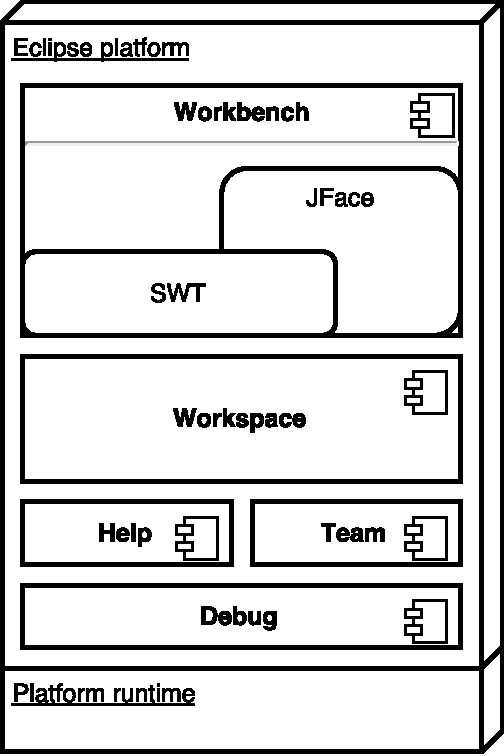
\includegraphics[width=0.5\textwidth, center]{obrazky-figures/eclipse_arch.pdf}
    \caption{Architektura platformy Eclipse.}
    \label{fig:eclipse_arch}
  \end{figure}

    \subsection{Workbench}
    %*********************
    Termín Workbench odkazuje na desktopové vývojové prostředí. Jeho cílem je integrace různých nástrojů a poskytnutí základního schématu pro tvorbu, správu a navigaci ve zdrojích pracovní plochy. Běžně se ve Workbench nachází lišta s hlavním menu, nástrojová lišta a několik pohledů, případně editorů\cite{eclipse-workbench}. Grafické prvky vývojového prostředí jsou však pro uživatele přizpůsobitelné.

    \begin{figure}[h]
      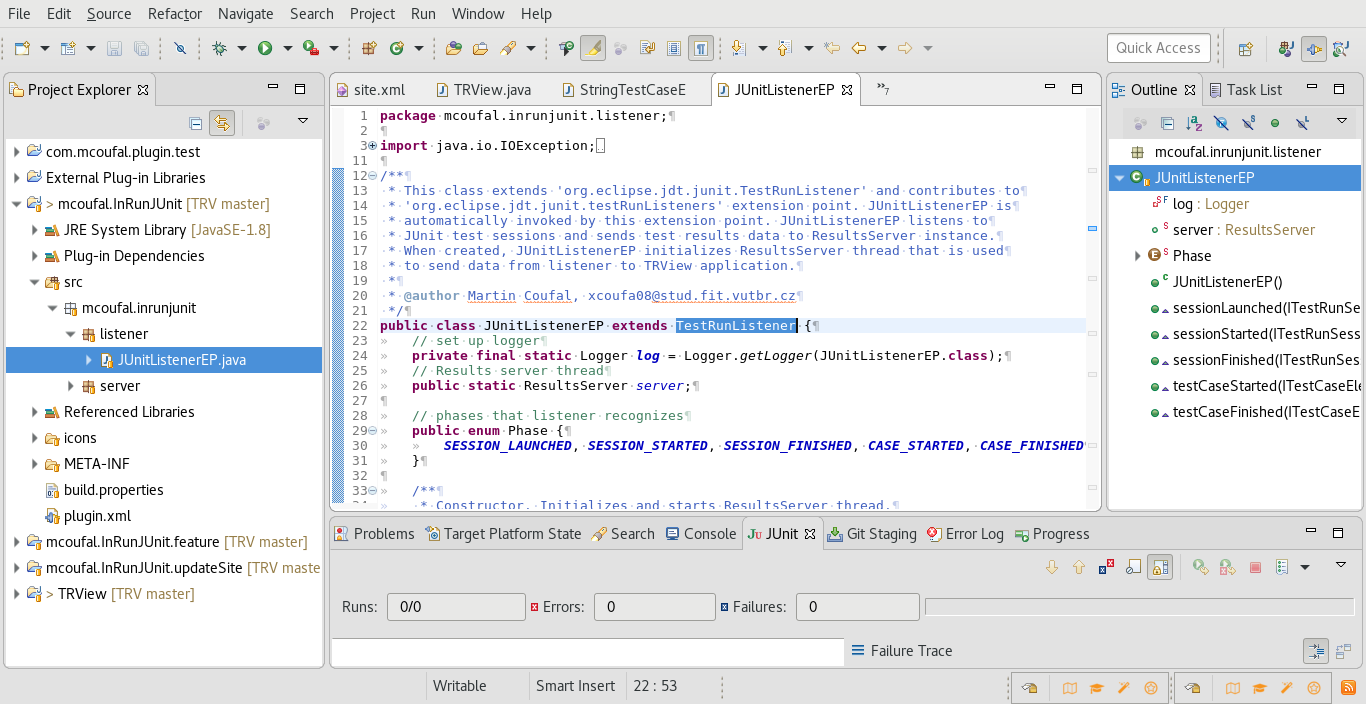
\includegraphics[width=0.7\textwidth, center]{obrazky-figures/eclipse_workbench.png}
      \caption{Běžný vzhled Eclipse Workbench.}
      \label{fig:eclipse_workbench}
    \end{figure}

      \subsubsection{Pohledy}
      %----------------------
      Pohled je jednou ze základních komponent tvořících uživatelské rozhraní Eclipse. Slouží k zobrazování zdrojových souborů a informací uživateli a také k navigaci ve vývojovém prostředí. Každý pohled může mít svá menu a své nástrojové lišty.
      
      Pro vytvoření nového pohledu je zapotřebí dvou kroků\,--\,vytvoření kategorie pohledu (pokud ho nechceme vytvořit v některé z již existujících kategorií) a deklarace nového pohledu. Obě dvě změny probíhají v manifestu zásuvného modulu. Přesto, že je možné tyto změny do manifestu dopsat ručně, vývojové prostředí Eclipse nabízí praktické nástroje pro editaci manifestů zásuvných modulů. Otevření některého z manifestů zásuvného modulu spustí editor zásuvného modulu. Nastavení rozšíření zásuvného modulu lze upravovat v záložce \emph{Extensions}. Pro přidání kategorie pohledu i deklarace pohledu samotného je nutné nejdříve přidat správný bod rozšíření. Všechny pohledy se připojují na bod rozšíření \texttt{org.eclipse.ui.views}. K tomuto bodu rozšíření lze přidat novou kategorii pohledu, nebo deklarovat nový pohled.

      Běžně používanou třídou implementující toto rozhraní je \texttt{org.eclipse.ui.part.ViewPart}. Zdrojový kód s popisem chování daného pohledu se nachází ve třídě implementující rozhraní \texttt{org.eclipse.ui.IViewPart}.

      \subsubsection{Perspektivy}
      %--------------------------
      Perspektivy slouží jako nástroj pro seskupení relevantních komponent v aktivním okně Workbench. Komponenty se seskupují podle úkonu, který bude uživatel vykonávat a  zároveň podle programovacího jazyka, ve kterém uživatel projekt vytváří. Eclipse IDE umožňuje přídání nových perspektiv pomocí zásuvných modulů a bodů rozšíření. Pokud je to žádoucí, lze také při přidání nového zásuvného modulu některou z již existujících perspektiv pouze upravit.

      Pro přidání nové perspektivy, podobně jako u přidání nového pohledu, je nutno do manifestu zásuvného modulu přidat správný bod rozšíření\,--\,\texttt{org.eclipse.ui.perspectives}. Rozložení komponent v dané perspektivě je definováno ve třídě implementující rozhraní \texttt{IPerspectiveFactory}. Přidat nové rozšíření zásuvného modulu implementující novou nebo upravenou perspektivu lze jednoduše pomocí nástrojů v záložce \emph{Extensions} u editoru zásuvného modulu. Chceme-li perspektivu pouze upravit, lze při tvorbě nové perspektivy vybrat některou z již existujících.

      \subsubsection{Editory}
      %----------------------
      Editory slouží jako hlavní nástroj pro úpravu zdrojového kódu a jiných textových souborů. Eclipse IDE nabízí mnoho editorů, které je možno nainstalovat v rámci nějakého ze zásuvných modulů. Nejzákladnějším editorem je textový editor. Ten poskytuje pouze základní funkce pro práci s textem bez zvýraznění nebo kontroly syntaxe. I ten je však možno dále rozšířit pomocí dalších zásuvných modulů.

      Editor lze přidat pomocí rozšiřujícího bodu \texttt{org.eclipse.ui.editors}. Na ten lze připojit vlastní třídu implementující rozhraní \texttt{org.eclipse.ui.IEditorPart}. Proces vytváření nového editoru je stejný jako v předchozích dvou případech.

    \subsection{SWT}
    %***************
    \todo{Popsat SWT? Je to vubec treba?}

  \section{Architektura zásuvných modulů v Eclipse IDE}
  %====================================================
  Každý zásuvný modul v Eclipse IDE slouží buď jako knihovna pro dodatečné funkce jiným zásuvným modulům, nebo slouží pro rozšíření funkcionality platformy. Chování každého zásuvného modulu je popsáno v jeho zdrojovém kódu. Závislosti, body rozšíření a služby poskytované  zásuvným modulem jsou popsány v manifestech modulu- souborech \texttt{MANIFEST.MF} a \texttt{plugin.xml}. Načítání nových zásuvných modulů probíhá až když je modul přímo vyžadován (dle návrhového vzoru lazy-loading). V základu jsou načteny pouze manifesty zásuvných modulů. Ty poskytují základní informace o zásuvném modulu a nemusí se tak načítat kompletní instalované zásuvné moduly. Díky tomuto modelu je Eclipse IDE i přes velké množství možných instalovaných zásuvných modulů kompaktnější a výrazně rychlejší při startu.

  Zásuvný modul (ať už v podobě Java archivu JAR nebo v podobě adresáře) se skládá z Javových tříd, manifestů zásuvného modulu (\texttt{MANIFEST.MF} a \texttt{plugin.xml}) a obrázkových souborů, typicky umístěných v adresářích pojmenovaných \emph{icons} nebo \emph{images}. Pokud je zásuvný modul ve formě adresáře, archiv JAR je uložen v některém z podadresářů. Název archivu JAR a jeho umístění je potom definováno v souboru \texttt{MANIFEST.MF}.

    \subsection{Model zásuvných modulů}
    %********************************
    Eclipse IDE při startu prohledá všechny adresáře se zásuvnými moduly a vytvoří vlastní model obsahující každý nalezený zásuvný modul. Tento model se vytváří pomocí manifestů zásuvných modulů tak, aby Elipse nemusel načítat celé zásuvné modely a ušetřil tak čas a místo. Informace o jednotlivých nainstalovaných zásuvných modulech jsou uloženy v balíčcích (\emph{angl. bundles}). Získáváním informací přes rozhraní těchto balíčků zajistíme, aby se zásuvné moduly nenačítaly, dokud nejsou opravdu zapotřebí.
    
    Původně mělo Eclipse IDE vlastní mechanismus pro běh aplikace, ale to znemožnilo použití již vytvořených technologií v jiných oblastech jako Avalon nebo JMX. Proto byl nakonec nahrazen mechanismem pro běh aplikace založeném na technologii OSGi Alliance, která poskytuje model s detailní specifikací a podporuje dynamické chování.\cite{Plugins}

    \subsection{Manifesty zásuvného modulu}
    %**************************************
    Manifesty zásuvného modulu jsou dva soubory\,--\,\texttt{MANIFEST.MF} a \texttt{plugin.xml}. První zmíněný obsahuje data nutná pro běh zásuvného modulu jako jsou \emph{identifikátor}, \emph{verze} a \emph{závislosti} zásuvného modulu. Druhý obsahuje data ve formátu XML popisující případná rozšíření a body rozšíření.

      \subsubsection{Manifest 'MANIFEST.MF'}
      %-------------------------------------
      V každém souboru \texttt{MANIFEST.MF} zásuvného modulu se nacházejí záznamy pro jméno, identifikátor, verzi, spouštěč a poskytovatele balíčku zásuvného modulu. Dále se zde mohou vyskytovat záznamy s cestou k knihovnám (\emph{ClassPath}), exportovanými balíčky a závislostmi zásuvného modulu.

      Jméno (\emph{Bundle-Name}) a poskytovatel (\emph{Bundle-Vendor}) jsou \emph{human-readable}\footnote{\url{https://en.oxforddictionaries.com/definition/us/human-readable}} řetězce, které nemusí být unikátní a lze je ukládat do zvláštního souboru \texttt{plugin.properties} za účelem internacionalizace.

      Identifikátor (\emph{Bundle-SymbolicName}) slouží k jednoznačné identifikaci daného balíčku. Většinou se jako identifikátor balíčku používá Javová konvence pro pojmenování balíčků: \texttt{com.<název společnosti>.<komponenta>[.<část komponenty>]}, kde část dané komponenty (například '\texttt{ui}' nebo '\texttt{core}') se uvádí v případě větších komponent, kde jsou jednotlivé balíčky rozděleny.
      
      Verze (\emph{Bundle-Version}) slouží k jednoznačné identifikaci verze daného balíčku. V případě shody identifikátorů je vždy vybrán balíček s novějším číslem verze. Toto číslo se skládá ze 3 číslic oddělených tečkami a v případě potřeby i alfanumerického řetězce použitelného pro užší specifikaci (například '\texttt{1.2.3.beta}'). První číslo označuje majoritní verzi produktu, druhé minoritní verzi produktu a třetí slouží k označení úrovně služeb.\todo{cituj me}

      Spouštěč (\emph{Bundle-Activator}) je volitelná část manifestu která umožňuje specifikovat třídu implementující rozhraní \texttt{BundleActivator} a poskytuje tak metody \texttt{start()} a \texttt{stop()}, které jsou přínosné pro správu životního cyklu balíčku.

      Cesta k knihovnám (\emph{Bundle-ClassPath}) je čárkami oddělený seznam knihoven ve formátu JAR obsahujících zdrojový kód zásuvného modulu.

      Záznam s exportovanými balíčky (\emph{Export-Package}) je podmnožina z cesty k knihovnám obsahující ty knihovny, které se mají exportovat, aby byly viditelné pro ostatní zásuvné moduly.

      \todo{Nasledujici text zni nejak zmatene}

      Eclipse IDE vytváří pro každý načtený zásuvný modul novou instanci pro načtení třídy, která slouží k vyhledávání a načítání zásuvných modulů a používá záznam závislostí v manifestu k určení viditelnosti ostatních zásuvných modulů. Záznam závislostí (\emph{Require-Bundle}) je seznam zásuvných modulů, které jsou pro daný zásuvný modul viditelné z hlediska vykonávání programu.

      \subsubsection{Manifest 'plugin.xml'}
      %------------------------------------
      V tomto manifestu zásuvného modulu mohou být uvedeny body rozšíření, na které je možno připojit nový zásuvný modul rozšiřující stávající funkcionalitu. Toto odloučení od rozšiřujících zásuvných modulů umožňuje existenci základního zásuvného modulu bez znalosti jakýchkoliv informací o ostatních zásuvných modulech. To zajišťuje snazší spolupráci při implementaci a znovupoužitelnost již implementovaných částí. Bod rozšíření obvykle definuje identifikátor, jméno a schéma. To určuje, co musí rozšiřující zásuvný modul splnit pro správné rozšíření tohoto zásuvného modulu.
      
      \todo{Přidat sample kódu jak vypadá rozšiřující bod.}
      
      \begin{figure}[!h]
	
\includegraphics[width=\textwidth, center]{obrazky-figures/placeholder.pdf}
	\caption{Zdrojový kód definující bod rozšíření.}
	\label{fig:plugins_extension_point}
      \end{figure}
      
      Dále je zde možno definovat, který zásuvný modul chceme stávajícím modulem rozšířit. K tomu slouží rozšíření zásuvného modulu (viz \ref{fig:plugins_extend_point})
      
      \begin{figure}[!h]
	
\includegraphics[width=\textwidth, center]{obrazky-figures/placeholder.pdf}
	\caption{Zdrojový kód definující, ke kterému bodu rozšíření se chceme připojit.}
	\label{fig:plugins_extend_point}
      \end{figure}

%=========================================================================%
% - - - KAPITOLA 3: J U N I T                                             %
\chapter{JUnit}                                                           %
%=========================================================================%
\todo{Popsat více do detailu, přidat odkaz na nástroje rozšiřující JUnit.}

JUnit je jednoduchý nástroj pro psaní testů a testování aplikací. Jeho vývoj je založen na otevřeném zdrojovém kódu (\emph{angl. open-source}), a proto lze najít další nástroje, které rámec JUnit používají nebo z něj vycházejí. Cílem JUnit je poskytovat nástroj, který umožní:
\begin{description}
  \item[Jednoduchost psaní testů]
  Programátor nemusí psát zbytečně mnoho kódu, zbytek za něj vykoná rámec JUnit.
  \item[Snadné pochopení rámce JUnit]
  Lorem ipsum dolor sit amet.
  \item[Rychlé provedení testů]
  Lorem ipsum dolor sit amet.
  \item[Izolované provedení testů]
  Lorem ipsum dolor sit amet.
  \item[Skládat a provádět různé kombinace testů]
  Lorem ipsum dolor sit amet.
\end{description}

Bohužel jsou některé z těchto podmínek v rozporu mezi sebou a tak nelze splnit všechny z těchto požadavků naplno.
  
  \section{Architektura rámce JUnit}
  %=================================
  Lorem ipsum dolor sit amet.

    \subsection{xUnit}
    %*****************
    % Vychazi z xUnit - popsat navrh xUnit + jak vynikl SUnit (odkaz na praci K. Becka Simple Smalltalk Testing: With Patterns)
    Lorem ipsum dolor sit amet.

    \subsection{JUnit}
    %*****************
    % Popis architektury / implementace JUnit 
    Lorem ipsum dolor sit amet viz obr \ref{fig:junit_arch}.

    \begin{figure}[!h]
      
\includegraphics[width=\textwidth, center]{obrazky-figures/placeholder.pdf}
      \caption{Architektura testovacího rámce JUnit.}
      \label{fig:junit_arch}
    \end{figure}

  \section{Rozšíření rámce JUnit}
  %==============================
  Lorem ipsum dolor sit amet.

  \section{Zásuvné moduly Eclipse IDE rozšiřující rámec JUnit}
  %===========================================================
  Lorem ipsum dolor sit amet.
  % Zminit jake moduly rozsiruji JUnit a jak, detailneji popsat jen ten co pouziji.
    \subsection{Zásuvný modul org.junit.???}
    %***************************************
    Lorem ipsum dolor sit amet.
    \subsubsection{JUnit ui}
    %-----------------------
    % Tady by mela byt popsana zakladni struktura daneho pluginu + Tridy dulezite z hlediska implementace 
    Lorem ipsum dolor sit amet.
    \subsubsection{JUnit core}
    %-------------------------
    % Tady by mela byt popsana zakladni struktura daneho pluginu + Tridy dulezite z hlediska implementace
    Lorem ipsum dolor sit amet.

%=========================================================================%
% - - KAPITOLA 4: Z Á S U V N Ý - M O D U L - I n R u n J U n i t V i e w %
\chapter{Implementovaná aplikace TestRunView}                             %
%=========================================================================%
Díky architektuře zásuvných modulů je snadné rozšířit Eclipse IDE o novou funkcionalitu a tak poskytuje četné množství prvků, které je vhodné otestovat. V rámci testování GUI Eclipse IDE se používají rozsáhlé testovací sady testující velké množství aspektů a možností. Automatické testy GUI jsou ale časově náročné a nejsou dokonalé. Vzniká tak potřeba kontroly nad sadou s probíhajícími testy. Průběh testů lze sledovat pomocí zásuvného modulu \texttt{org.eclipse.jdt.junit}, který poskytuje pohled JUnit zobrazující potřebné informace o probíhajících testech. Navíc umožňuje znovu spustit testovací sadu a také si uchovává historii testovaných sad. Problémem tohoto pohledu je, že při spuštění testovací sady se otevírá nové okno s testovanou instancí Eclipse IDE. To způsobí překrytí pohledu JUnit a proto není možné sledovat tento pohled v průběhu testování. Také z hlediska časové náročnosti může být výhodnější testovat na vzdálených serverech a spouštět testy z terminálu. V takovém případě nelze pohled JUnit k zobrazení detailů o testování použít.

Implementovaná aplikace \emph{TestRunView} (dále zkráceně TRV) poskytuje možnost zobrazení informací o probíhajícím testování GUI Eclipse IDE bez narušení průběhu testů. Mezi důležité informace které tato aplikace zobrazuje patří zobrazení průběhu a výsledků jednotlivých testovacích případů v rámci spuštěné testovací sady. V případě nějaké chyby v testovací sadě potom lze lépe prozkoumat kde chyba nastala a napravit ji.

Tato kapitola detailně popisuje architekturu, implementaci, způsob testování a využití této aplikace.

  \section{Návrh architektury aplikace TestRunView}
  %================================================
  %TODO: jake reseni a proc sem vybral
  V rámci návrhu bylo třeba zvážit způsoby, jakými lze data o probíhajících testech získávat a jakými lze tyto data zobrazovat. Ve společnosti Red Hat Czech se používají pro testování rámce JUnit a \textit{RedDeer}\footnote{\url{https://github.com/jboss-reddeer}}. RedDeer je rámec pro testování zásuvných modulů Eclipse a využívá k tomu rámec JUnit. Pomocí implementace vlastního \emph{runneru} dostává kontrolu nad probíhajícími testy. To umožňuje definovat například pořadí a typ spuštěných testů, nebo vytvářet vlastní anotace a tak definovat nové fáze probíhající v rámci testování.

  Data tedy lze získávat jak z obou zásuvných modulů\,--\,JUnitu i RedDeeru. JUnit ovšem narozdíl od RedDeeru poskytuje možnost připojit se pomocí bodu rozšíření \texttt{\todo{BOD}} a tak umožňuje širší použití výsledné aplikace. Vytvořený zásuvný modul není třeba explicitně přidávat v kódu rámce nebo testů, ale je automaticky spuštěn.
  \\
  \\
  \noindent
  Možností jak zobrazit tyto informace je několik:
  \begin{itemize}
   \item pohled (nebo jiná komponenta Eclipse Workbench) přímo v instanci Eclipse IDE s běžícími testy
   \item v externí aplikaci
   \item pomocí nástrojů operačního systému (notifikace, terminál)
  \end{itemize}

  Při zobrazování dat je nutné aby nedocházelo k narušování běhu testů a zároveň byly informace o běžících testech viditelné. V případě zobrazování informací o probíhajících testech přímo v testované instanci Eclipse IDE by bylo velmi problematické zajistit oba tyto případy. Zobrazení informaci pomocí nástrojů operačního systému by sice umožňovalo nenarušený běh testů, ale přehlednost zobrazených výsledků by byla nižší. Proto je zobrazení výsledků implementováno pomocí externí SWT aplikace, která umožňuje nenarušený průběh testů a komfortní zobrazení výsledků.

  Velmi důležitou částí návrhu je způsob předávání dat mezi částí získávající informace o testech a částí, která tyto informace zobrazuje. To lze řešit například externím souborem nebo pomocí síťové komunikace typu klient-server. V aplikaci je z důvodu možnosti připojení klientské aplikace k vzdálenému serveru zvolen způsob komunikace typu klient-server.

  Aplikace TRV se skládá ze dvou částí\,--\,zásuvného modulu InRunJUnit a SWT aplikace TRView\,(viz Obrázek \ref{fig:TRV_architecture}). InRunJUnit je nainstalován jako jeden ze zásuvných modulů Eclipse a slouží k získání a zpracování výsledků ze zásuvného modulu JUnit. Zároveň slouží jako server, ke kterému lze připojovat klientské aplikace. TRView zpracovává a zobrazuje data o probíhajících testech uživateli. Tyto data získává pomocí soketů přijatých ze serveru.

  \begin{figure}[!h]
    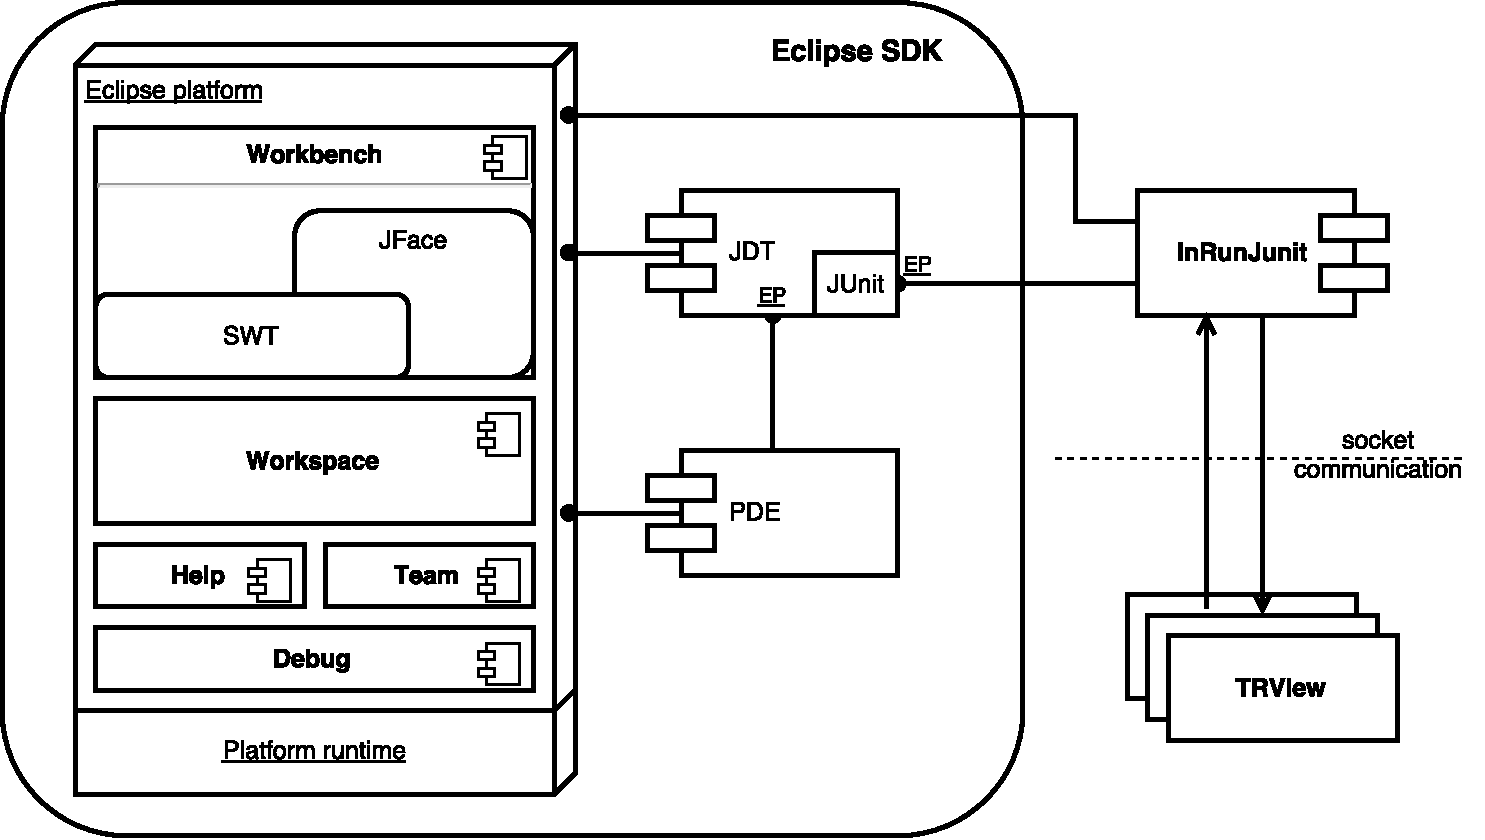
\includegraphics[width=\textwidth, center]{obrazky-figures/TRV_architecture.pdf}
    \caption{Znázornění architektury aplikace TRV.}
    \label{fig:TRV_architecture}
  \end{figure}

    \subsection{Návrh architektury zásuvného modulu InRunJUnit}
    Integrace zásuvného modulu InRunJUnit do platformy Eclipse je znázorněna na obrázku \ref{fig:inrunjunit_eclipse_integration}. Zásuvný modul se skládá ze dvou částí\,--\,\emph{listeneru} a serveru. Listener je pomocí bodu rozšíření poskytovaného zásuvným modulem JUnit zaregistrován mezi ostatní listenery. Poté, co se spustí JUnit za účelem testování, si JUnit zjistí které zásuvné moduly jsou k bodu rozšíření připojeny a automaticky je informuje o průběhu testů. Server se stará o vytvoření serveru, komunikaci s klienty, vytvoření relevantních dat ve formě řetězce a jejich posílání všem připojeným klientům. Při posílání dat také specifikuje fázi testování\footnote{Může se jednat o zahájení (případně ukončení) testovací sady nebo testovacího případu.}, ze které data pochází.

      \begin{figure}[!h]
	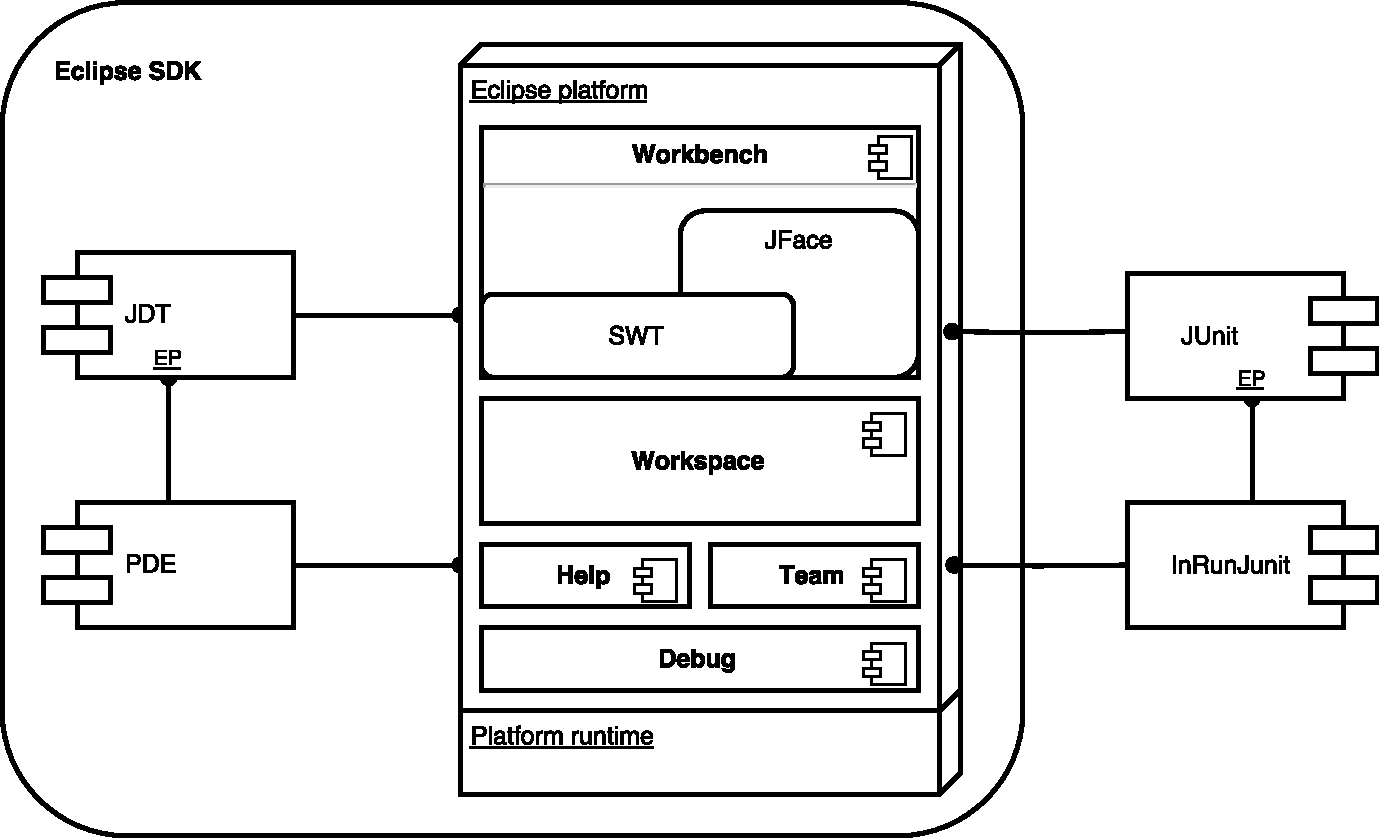
\includegraphics[width=\textwidth, center]{obrazky-figures/inrunjunit_eclipse_integration.pdf}
	\caption{Znázornění integrace zásuvného modulu InRunJUnit v platformě Eclipse.}
	\label{fig:inrunjunit_eclipse_integration}
      \end{figure}

    \subsection{Návrh architektury aplikace TRView}
    Aplikace TRView se také skládá ze dvou částí\,--\,klienta a zobrazení. Klientská část umožňuje připojení k serveru a ukládání přijatých výsledků. Při přijetí dat ze serveru také inicializuje zpracování a zobrazení průběhu testů do GUI. Část zobrazení se stará o vytvoření a obsluhu grafického rozhraní. GUI obsahuje komponenty, které slouží pro připojení k serveru a zobrazují důležité informace o průběhu testů. To zahrnuje:
    \begin{itemize}
     \item pole pro zadání adresy a portu serveru
     \item počet testovacích případů, které poběží
     \item počet testových chyb v testech
     \item počet běhových chyb v testech
     \item počet přeskočených testů
     \item stromovou strukturu jednotlivých testovacích případů s:
     \begin{itemize}
      \item rozlišením který test je aktivní
      \item rozlišením výsledku testovacího případu
      \item časem udávajícím trvání testovacího případu
     \end{itemize}
     \item zobrazení \emph{stack strace} pro neúspěšné testy
    \end{itemize}

    V případě, že testy a klientská aplikace poběží na jednom systému, je třeba vzít v úvahu problém aktivního okna. Některé testy vyžadují pro nalezení a otestování komponent aktivitu daného okna. To může způsobit překrytí okna aplikace TRView a tak znemožnit zobrazení informací o probíhajících testech uživateli. Proto je okno aplikace TRView vytvořeno \uv{vždy nahoře}(\emph{angl. always on top}). Okno tak bude vždy viditelné, i když nebude aktivní.

    \subsection{Integrace zásuvného modulu InRunJUnit a SWT aplikace TRView}
    \todo{Lorem ipsum dolor sit amet.}

  \section{Implementace aplikace TRV}
  %==================================
  \todo{Lorem ipsum dolor sit amet.}

    \subsection{Implementace zásuvného modulu InRunJUnit}
    \todo{Lorem ipsum dolor sit amet.}
    \subsection{Implementace aplikace TRView}
    \todo{Lorem ipsum dolor sit amet.}
    \subsection{Implementace komunikace InRunJUnit a TRView}
    \todo{Lorem ipsum dolor sit amet.}
  
  \section{Testování}
  %==================
  \todo{Lorem ipsum dolor sit amet.}

    \subsection{Jednotkové testování}
    \todo{Lorem ipsum dolor sit amet.}
    \subsection{Integracni testovani}
    \todo{Lorem ipsum dolor sit amet.}

  \section{Praktické využití}
  %=========================
  \todo{Lorem ipsum dolor sit amet.}

    \begin{figure}[!h]
	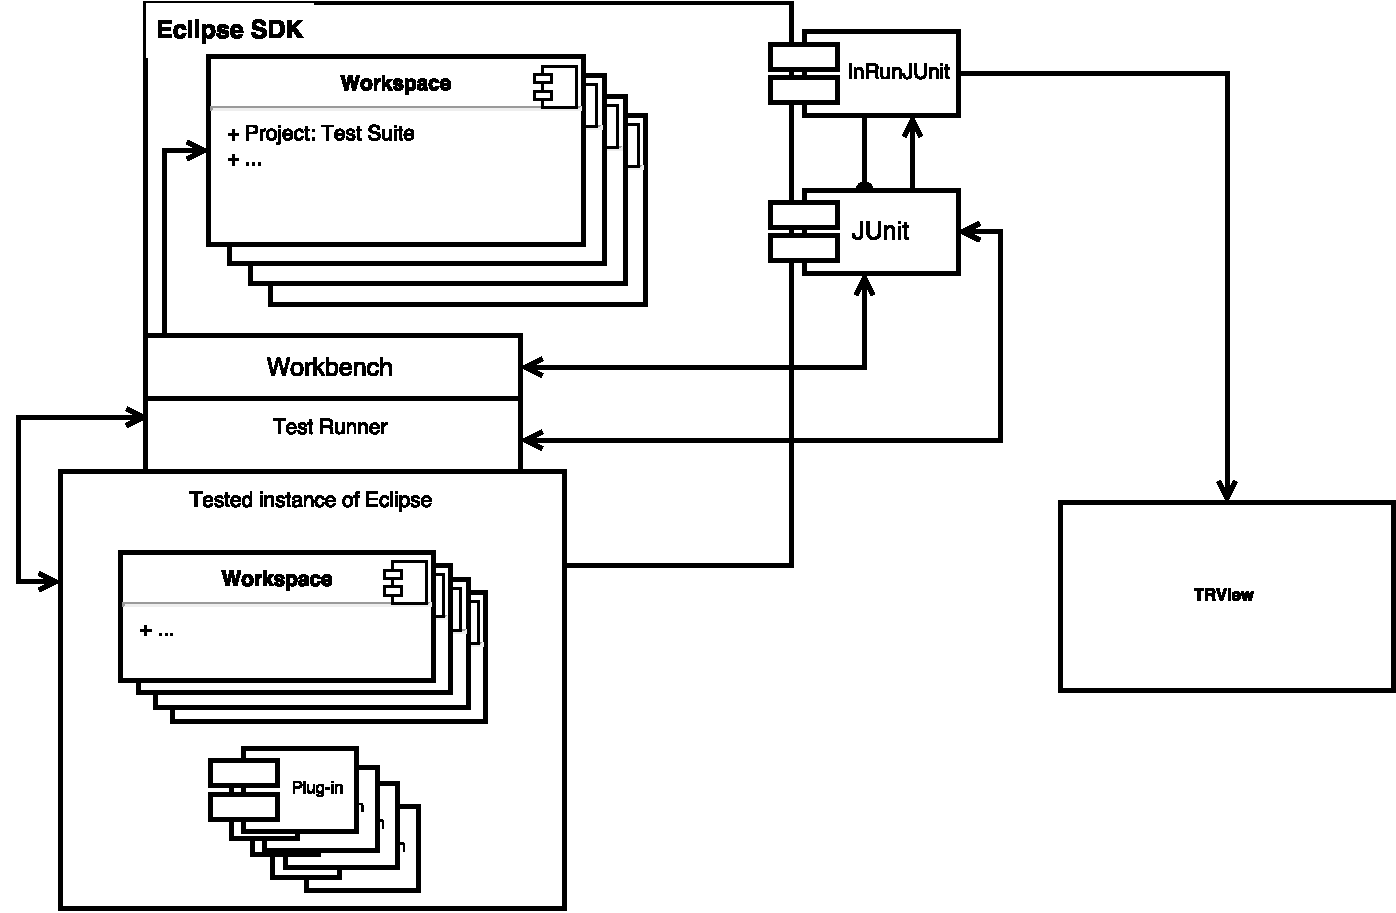
\includegraphics[width=\textwidth, center]{obrazky-figures/TRV_run_from_gui.pdf}
	\caption{Znázorňění funkce aplikace TRV při spuštění testů z GUI Eclipse IDE.}
	\label{fig:TRV_run_from_gui}
      \end{figure}

    \subsection{Použití při testování Eclipse IDE v~RedHat}
    %**************************************************
    Lorem ipsum dolor sit amet.

    \begin{figure}[!h]
	
\includegraphics[width=\textwidth, center]{obrazky-figures/placeholder.pdf}
	\caption{Znázorňění funkce aplikace TRV při spuštění testů z terminálu.}
	\label{fig:TRV_run_from_term}
      \end{figure}

    \subsection{Jiná využití}
    %************************
    Lorem ipsum dolor sit amet.

  \section{Možná rozšíření}
  %========================
  Lorem ipsum dolor sit amet.

%=========================================================================%
% - - - KAPITOLA 5: Z Á V Ě R                                             %
\chapter{Závěr}                                                           %
%=========================================================================%
Závěrečná kapitola obsahuje zhodnocení dosažených výsledků se zvlášť vyznačeným vlastním přínosem studenta. Povinně se zde objeví i zhodnocení z~pohledu dalšího vývoje projektu, student uvede náměty vycházející ze zkušeností s~řešeným projektem a uvede rovněž návaznosti na právě dokončené projekty.

%=========================================================================
 % viz. obsah.tex / see obsah.tex

  % Pouzita literatura / Bibliography
  % ----------------------------------------------
\ifslovak
  \makeatletter
  \def\@openbib@code{\addcontentsline{toc}{chapter}{Literatúra}}
  \makeatother
  \bibliographystyle{bib-styles/czechiso}
\else
  \ifczech
    \makeatletter
    \def\@openbib@code{\addcontentsline{toc}{chapter}{Literatura}}
    \makeatother
    \bibliographystyle{bib-styles/czechiso}
  \else 
    \makeatletter
    \def\@openbib@code{\addcontentsline{toc}{chapter}{Bibliography}}
    \makeatother
    \bibliographystyle{bib-styles/englishiso}
  %  \bibliographystyle{alpha}
  \fi
\fi
  \begin{flushleft}
  \bibliography{xcoufa08-Pohled-na-stav-JUnit-pro-testovanou-instanci-eclipse-20-literatura-bibliography}
  \end{flushleft}

  % vynechani stranky v oboustrannem rezimu
  % Skip the page in the two-sided mode
  \iftwoside
    \cleardoublepage
  \fi

  % Prilohy / Appendices TODO: Uncomment appendix, appendixpage, startcontents[chapter] if appendices pressent
  % ---------------------------------------------
  %\appendix
\ifczech
  \renewcommand{\appendixpagename}{Přílohy}
  \renewcommand{\appendixtocname}{Přílohy}
  \renewcommand{\appendixname}{Příloha}
\fi
\ifslovak
  \renewcommand{\appendixpagename}{Prílohy}
  \renewcommand{\appendixtocname}{Prílohy}
  \renewcommand{\appendixname}{Príloha}
\fi
  %\appendixpage

% vynechani stranky v oboustrannem rezimu
% Skip the page in the two-sided mode
\iftwoside
  \cleardoublepage
\fi
  
\ifslovak
%  \section*{Zoznam príloh}
%  \addcontentsline{toc}{section}{Zoznam príloh}
\else
  \ifczech
%    \section*{Seznam příloh}
%    \addcontentsline{toc}{section}{Seznam příloh}
  \else
%    \section*{List of Appendices}
%    \addcontentsline{toc}{section}{List of Appendices}
  \fi
\fi
  %\startcontents[chapters]
  % seznam příloh / list of appendices
  % \printcontents[chapters]{l}{0}{\setcounter{tocdepth}{2}}
  
  % vynechani stranky v oboustrannem rezimu
  \iftwoside
    \cleardoublepage
  \fi
  %\chapter{Obsah přiloženého paměťového média}
\label{jak}

\begin{itemize}
 \item {\LARGE \textbf{TRV/:} kořenový adresář.}
    {\Large \begin{itemize}
     \item \textbf{mcoufal.InRunJUnit:}
	Adresář obsahující zdrojové soubory implementovaného zásuvného modulu InRunJUnit.
     \item \textbf{mcoufal.InRunJUnit.feature:}
	Adresář obsahující feature projekt se zásuvným modulem InRunJUnit.
     \item \textbf{mcoufal.InRunJUnit.updateSite:}
	Adresář obsahující update site projekt se zásuvným modulem InRunJUnit.
     \item \textbf{README.md:}
	Soubor popisující základní použití a instalaci vytvořeného nástroje TRV.
     \item \textbf{technical-report:}
	Adresář obsahující zdrojové soubory použité pro tvorbu této práce.
     \item \textbf{TRView:}
	Adresář obsahující zdrojové soubory aplikace TRView a spustitelný JAR archiv \texttt{TRView.jar}.
     \item \textbf{xcoufa08-Pohled-na-stav-JUnit-pro-testovanou-instanci-eclipse.pdf:}
	Soubor ve formátu PDF obsahující elektronickou verzi této práce.
    \end{itemize}}
\end{itemize}


 % viz. prilohy.tex / see prilohy.tex TODO: uncomment if any appendices pressent
\end{document}
